%%% Lecture 4

\lecture[We finish the proof of the HAT. My first non-trivial homotopy groups.]{2021-10-25}
$(k\geq2)$ Set $u_i=f_i(\text{center of } I^n)\in I^n$. Assume without loss of generality that the first coordinates of $\nn{u}{k}$ are not all equal (if some of them are, we can "wiggle" $f_1$).

\begin{center}
\begin{tikzpicture}[x=0.7em, y=0.7em, baseline=0.7*5em]
\filldraw[very thick, black, fill=blue!20]
    (0,0)--(0,10)--(10,10)--(10,0)--(0,0);
\filldraw[fill=white, use Hobby shortcut,closed=true] 
    (1,5) .. (4,9) .. (7,5) .. (4,8) .. (3,4) .. (5,2) .. (7,5) .. (8,2) .. (5,1);
\filldraw[fill=white, use Hobby shortcut,closed=true] 
    (4,5) .. (4,6) .. (5.3,6) .. (5.4,4);
\filldraw[fill=white, use Hobby shortcut,closed=true] 
    (8,1) .. (8,2) .. (9,2) .. (9,1);
\draw 
    (7,6) node {\scriptsize$f_1$}
    (8.5,1.5) node {\scriptsize$f_2$}
    (5.2,4.9) node {\scriptsize$f_3$};
\end{tikzpicture}
$\xrightarrow{\text{shrink domains to}}$
\begin{tikzpicture}[x=0.7em, y=0.7em, baseline=0.7*5em]
\filldraw[very thick, black, fill=blue!20]
    (0,0)--(0,10)--(10,10)--(10,0)--(0,0);
\filldraw[fill=white, use Hobby shortcut,closed=true] 
    (1,5) .. (2,6) .. (3,5) .. (2.5,3);
\filldraw[fill=white, use Hobby shortcut,closed=true] 
    (4,5) .. (4,6) .. (5.3,6) .. (5.4,4);
\filldraw[fill=white, use Hobby shortcut,closed=true] 
    (8,1) .. (8,2) .. (9,2) .. (9,1);
\draw[dashed] (3.5,0)--(3.5,10) (6.5,0)--(6.5,10);
\draw 
    (2,5) node {\scriptsize$f_1$}
    (8.5,1.5) node {\scriptsize$f_2$}
    (5.2,4.9) node {\scriptsize$f_3$};
\end{tikzpicture}
$\xrightarrow{\text{blow images to}}$
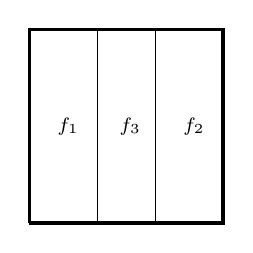
\begin{tikzpicture}[x=0.7em, y=0.7em, baseline=0.7*5em]
\draw[very thick, black]
    (0,0)--(0,10)--(10,10)--(10,0)--(0,0);
\draw (3.5,0)--(3.5,10) (6.5,0)--(6.5,10);
\draw 
    (2,5) node {\scriptsize$f_1$}
    (8.5,5) node {\scriptsize$f_2$}
    (5.2,5) node {\scriptsize$f_3$};
\end{tikzpicture}
\end{center}

\hspace*{\fill}$\leadsto [g] = \sum[g\circ f_i].$


Choose $t\in (0,1)$ such that
\begin{itemize}
    \item $t$ is different from the first coordinates of $\nn{u}{k}$,
    \item for some $1\leq i\leq k$, the first coordinate of $u_i$ is smaller than $t$,
    \item for some $1\leq i\leq k$, the first coordinate of $u_i$ is larger than $t$.
\end{itemize}

Choose neighborhoods $\Uu_i$ of $u_i$ inside $f_i(\ring I^n)$ that do not intersect $\cb{t}\times I^\ni$, that is such that $\Uu_i$ lies "on the same side respect to $t$" as $u_i$.

Choose subcubes $Q_i$ inside $\ring I^n$ that contain the center and lie in in $f^{-1}(\Uu_i)$.

Last time we proved that $g$ is pair-homotopic to some $g':\pair\to\pairs$ such that
\[g'(I^n\sm\bigcup_{i=1,\dots,k} f_i(Q_i))\subset A\quad\text{and}\quad[g\circ f_i]=[g'\circ f_i]\text{ in }\pi_n\pairs^\#.\]

We precompose each $f_i:I^n\to I^n$ with the linear shrinking homotopy relative $Q_i$. Set $f'_i=f_i\circ \text{ end of shrinking}$. Then $g'\circ f_i$ is pair homotopic to $g'\circ f'_i$ and $f'_i(I^n)\subset\Uu_i$.

By replacing $g$ by $g'$ and $f_i$ by $f'_i$ we can therefore assume without loss of generality that $f_i(\ring I^n)$ lies on one side of $\cb{t}\times I^\ni$.

\begin{center}
\begin{tikzpicture}[x=0.7em, y=0.7em, baseline=0.7*5em]
\filldraw[very thick, black, fill=blue!20]
    (0,0)--(0,10)--(10,10)--(10,0)--(0,0);
\filldraw[fill=white, use Hobby shortcut,closed=true] 
    (1,5) .. (2,6) .. (3,5) .. (2.5,3);
\filldraw[fill=white, use Hobby shortcut,closed=true] 
    (4,5) .. (4,6) .. (5.3,6) .. (5.4,4);
\filldraw[fill=white, use Hobby shortcut,closed=true] 
    (8,1) .. (8,2) .. (9,2) .. (9,1);
\draw[dashed] (3.5,0)--(3.5,10);
\draw 
    (2,5) node {\scriptsize$f_1$}
    (8.5,1.5) node {\scriptsize$f_2$}
    (5.2,4.9) node {\scriptsize$f_3$};
\end{tikzpicture}
\end{center}\smallskip

Write $g=g_1+_t g_2$ by "cutting along $\cb{x_1=t}$".

Formally, $g_1(\xs)=g(t\xs)$ and $g_2=g((1-t)x_1+t,\dots,x_n)$.

Set $I_1=\cb{i\in I\mid u_i\text{ lies left of }\cb{x_1=t}}$ and $I_2=\cb{i\in I\mid u_i\text{ lies right of }\cb{x_1=t}}$, where $I=\cb{1,\dots,k}$.

Then by the inductive hypothesis:
\[[g]=[g_1]+[g_2]=\sum_{i\in I_1}\deg(f_i)[g_1\circ f_i]+\sum_{i\in I_2}\deg(f_i)[g_2\circ f_i]=\sum_{i\in I}\deg(f_i)[g\circ f_i].\]\qed

\section{My First Non-Trivial Homotopy Group}

\begin{theorem}
Let $n\geq2$ and assume the HAT in dimension $n$. Then $\pi_n(S^n,*)$ is infinite cyclic.
\end{theorem}

\begin{proof}
Choose some point $z\in S^n$. Set $U=S^n\sm\cb{-z}$. Then \[\pi_n(S^n,z)=\pi_n(S^n,\cb{z},z)\underset{U\cong *}{\cong}\pi_n(S^n,U,z)\underset{\pi_1(U,z)=\cb{1}}{\cong}\pi_n(S^n,U,z)^\dagger\cong\pi_n(S^n,U)^\#\]
So we may show that $\pi_n(S^n,U)^\#\cong\Z$.

We show that $\pi_n(S^n,U)^\#$ is generated by the class of any pair map $\psi:\pair\to(S^n,U)$ such that $\psi(\de I^n)=\cb{z}$ and $\psi$ factors out a homeomorphism $I^n/\de I^n\cong S^n$.

Let $f:(I^n,\de I^n)\to(S^n,U)$ be any pair map. Set $V=S^n\sm\cb{z}$ so that $S^n=U\cup V$ is an open cover.

The Lebesgue Number lemma provides an $m\geq1$ so that each subcube of $I^n$ of side length $1/m$ is mapped by $f$ into $U$ or into $V$. Decompose $I^n$ into $m^n$ subcubes of side length $1/m$.

We define subspaces of $I^n$ in this way:
\begin{itemize}[label=-]
    \item $A_{-1}=\de I^n$
    \item $A_0=A_{-1}\cup\text{ vertices}$
    \item $A_1=A_0\cup\text{ edges}$
    \item $A_2=\cdots$
    \item $A_n=I^n$
\end{itemize}

We want to "improve" $f$ successively by pair homotopies to maps $f=f_{-1},f_0,f_1,\dots,f_{n-1}$ such that:
\begin{itemize}
    \item each $f_j$ is homotopic to $f$ relative $\de I^n$,
    \item each $f_j$ is admissible, i.e. it sends every subcube of side length $1/m$ to $U$ or to $V$,
    \item $f_j(A_j)\subset U$ for $j=-1,0,1,\dots,n-1$.
\end{itemize}

We proceed by induction on $j$. There is nothing to show for $j=-1$. Let now $j\geq 0$. We first modify $f_{j-1}$ and the faces of the $j$-cube. If such a face $Q$ is "good", i.e. sent by $f_{j-1}$ into $U$, we do not do anything to $Q$. Otherwise the $(j-1)$-subcube is mapped to $V$ and the restriction of $f_{j-1}$ to it is a pair map $(Q,\de Q)\to (V,V\cap U)$.

Claim. For $j<n$, any pair map $(I^j,\de I^j)\to (V,U\cap V)$ is homotopic relative $\de I^j$ to a map with image in $U\cap V$.

\begin{claimproof}
By stereographic projection $(U,U\cap V)$ is pair homotopic to $(\R^n,\R^n\sm\cb{0})$, i.e. we can costruct a pair map $g:(I^j,\de I^j)\to (\R^n,\R^n\sm\cb{0})$. Because $\de I^j$ is compact and $0\notin f(\de I^j)$, there is an $\epsilon>0$ such that $g(\de I^j)\cap(\epsilon\text{-ball around }0)=\emptyset$.

So $g:(I^j,\de I^j)\to(\R^n,\R^n\sm\ring B(\epsilon,0))$. Now, $\R^n$ can be obtained from $\R^n\sm\ring B(\epsilon,0)$ by attaching an $n$-cell. The cellular approximation theorem and the fact that $I^j$ is a $j$-dimensional CW-complex gives us a relative homotopy from $g$ to a cellular map. Since $j<n$, the cellular map has image in $\R^n\sm\ring B(\epsilon,0)\subset\R^n\sm\cb{0}$.
\end{claimproof}

We can now change $f_{j-1}|A_j$ into $f_j|A_j$ by a homotopy relative $A_{j-1}$ into a map that sends all $j$-cells to $U$.

We use the HEP for $(I^n,A_j)$ to extend $f_j$ to all of $I^n$; we use the HEP with target $U$ or with target $V$ to ensure that the map $f_j$ is again admissible.

After this inductive construction we can replace $f$ by $f_{n-1}$ and we have arranged without loss of generality that $f(A_{n-1})\subset U$.

We can now assume that $g:\pair\to(S^n,U)$ satisfies $g(A_{n-1})\subset U$ and each top-dimensional subcube is mapped to $U$ or to $V$.

We apply the HAT to this map $g$ with $\nn{f}{k}$ the reparametrization of those subcubes that are \textit{not} mapped into $U$ (and hence into $V$).

Then by the HAT we have:
\[[g]=\sum_i\pm[g\circ f_i]\text{ in }\pi_n(S^n,U)^\#\cong\pi_n(S^n,\cb{z},z)^\dagger\cong\pi_n(S,z)\]

We have gained that each summand on the right hand side is in the image of the homomorphism $\pi_n(V,V\cap U)^\#\to\pi_n(S^n,U)^\#$, which is then surjective. By the long exact homotopy group sequence of the pair $(V,V\cap U)$, we obtain:
\[\pi_n(V,V\cap U,z)=\pi_n(\R^n,\R^n\sm\cb{0},z)\cong\pi_\ni(\R^{n-1}\sm\cb{0},z)\cong\pi_\ni(S^\ni,z)\cong\Z\]
so $\pi_n(S^n,U)^\#$ is infinite cyclic.

\end{proof}

\section{Reminder on Simplicial Sets}

We denote by $\Delta$ the category with objects the sets $[n]=\cb{0,1,\dots,n}$, $n\geq 0$ and morphisms the weakly monotone maps.

A \textbf{simplicial set} is a contravariant functor from $\Delta$ to sets, $X:\Delta^\op \to\Set$. The set of the $n$-simplices is denoted $X_n=X([n])$, for a morphism $\alpha:[n]\to[m]$ write $\alpha^*=X(\alpha):X_m\to X_n$.

The \textbf{singular complex} (singular simplicial set) of a space $Y$ is the simplicial set \[\S(Y)=\{\text{all continuous maps }f:\nabla^n=\cb{(\xso)\in\R^{n+1}\mid x_i\geq0,\ \sum x_i=1}\to Y\}.\]

For $\alpha: [n]\to [m]$, the map $\alpha^*:\S(Y)_m\to\S(Y)_n$ is precomposition with the affine linear map $\alpha_*:\nabla^n\to\nabla^m$, $e_i\mapsto e_{\alpha(i)}$. 

For a continuous map $\psi:Y\to Z$, a morphism of simplicial sets $\psi_*=\S(f):\S(Y)\to\S(Z)$ is given by $\S(\psi)_n(f)=\psi\circ f$. This yelds a functor $\S:\Top\to\sSet$.

The \textbf{geometric realization} is a functor $|-|:\sSet\to\Top$ defined as follows. For a simplicial set $X$, $|X|=(\coprod X_n\times\nabla^n)/\sim$, where $X_n$ is endowed with the discrete topology and the equivalence relation is the one generated by:\normalmarginpar\marginnote{\footnotesize The equivalence relation is only \textit{generated} by the condition stated, which is not (what?). The actual equivalence relation is not easy to understand, apparently.}
\[X_m\times\nabla^m\cont(x,\alpha_*(t))\sim(\alpha^*(x),t)\in X_n\times\nabla^n\quad\text{for all }\alpha:[n]\to[m],\ x\in X_m,\ t\in\nabla^m.\]

\reversemarginpar
